% this file is called up by thesis.tex
% content in this file will be fed into the main document

\chapter{Social Testing} % top level followed by section, subsection
\label{ch:ST}

\begin{textsl}
{\small Continuous delivery (CD) and delivering software for the Cloud represents a challenge for software test teams, because of the continuous introduction of new features and feedback from customers.  In this chapter we consider two frameworks in the form of two case studies. The first where users are encouraged to report defects through social or other incentive schemes. The second, where field defect detection rates in a framework where these rates are used to refocus in-house test resources. Using two enterprise datasets, we address the following questions: what types of defects can best be found in the field, allowing in-house test resources to be refocused and how soon after a system goes live defects are detected. The benefit to small tests is two fold: minimise the number of defects found in the field by maximising internal usage through `Dogfood' programs, by leveraging crowdsourced test methodologies and by adopting a reward scheme to incentivise customers to fine low severity field defects.}
\end{textsl}

\vspace*{1cm}

%\adjustmtc

%\minitoc
% ----------------------- contents from here ------------------------


% % % % % % % % % % % % % % % % % % % % % % % % % % % % % % % % % % % % % % % % % % % % % % % % % % % % % %
%---------------------------------------- INTRODUCTION ----------------------------------------------------
% % % % % % % % % % % % % % % % % % % % % % % % % % % % % % % % % % % % % % % % % % % % % % % % % % % % % %
\section{Introduction}

** Social Testing Intro

Small to medium enterprises (SME's) are the backbone of the European economy representing 79\% of all employment with an annual turnover in excess of 440 billion Euro \cite{eurocom2014sme}. The European customer is maturing technologically and now demands more from their interaction with products and services. This has placed an additional challenge on the SME to provide products and services in a rapid and connected way. Nine out of ten SME's in Europe have less than ten employees \cite{eurocom2014sme} which makes it difficult for an SME to find the necessary additional capacity to cater for the new European customer.  CD is seen as one approach that can be readily adopted by the SME to help reduce the software delivery life cycle. CD promotes faster delivery of software components, features and fixes \cite{humble2010continuous}. With an accelerated delivery of product/service improvements, SME's want to keep pace with large enterprise solution providers.  In the race to provide solutions in a dynamic agile way, large enterprises have the resources to exploit CD. These same enterprises can also leverage fully mature software test teams to ensure a succession of stable releases for the consumer and reduce the risk of subsequent brand damage due to releasing a poor quality product or service. The adoption of CD is non-trivial.  Recent work has been conducted to outline the key challenges faced by software companies. These include: development of features rather than components and the development of an automated test harness to support testing \cite{olsson2012climbing}. An SME cannot compete at this level. \par

In this paper, we describe a framework, which the SME can leverage to best utilise their limited in-house test resources while utilising their greatest test asset: the customer. The core idea of this framework is for the in-house test teams to focus on high value test areas, while incentivising the customer to find   low impact field defects. This paper contains a study of software defect data from a large enterprise dataset. Through this study of customer defect data we show which types of defects the customer is useful at finding. By leveraging the customer's skill at finding certain categories of defects, we argue that incentivising the customer to find a particular class of defect, can aid the SME to deliver higher quality software by diverting in-house test resources to high value areas such as performance and systems testing. \par

For cloud-based systems where multi-tenancy is employed, defect data could be shared socially between customers to better understand component usage patterns and fault prone functionality. The rest of the paper is structured in five Sections; Section II gives some description of study background and related works. Section III describes the enterprise dataset. Section IV discusses the analysis and method and it is followed by section V which explains the result. Finally, the conclusion and future work is described in Section VI.


** Social Dogfood Intro

Cloud computing is seen as a way for an SMEs to compete with larger companies, in terms of the rapid delivery of software and services. This is due in part to the `always on' nature of Cloud computing. European SMEs are beginning to see the green shoots of economic recovery, in 2015 SME economic growth grew by 5.6\% \cite{europa2016sme}. Additionally SME employment growth grew by 1.5\% \cite{europa2016sme}. As the economic recovery continues SMEs are looking to maximise their potential. \par

However both micro-teams and SMEs face continuing challenges when adopting both Cloud computing and continuous delivery as their hosting and software delivery mechanisms respectively. A recent study has outlined the issues facing SMEs in adopting industry standards in relation to software development and delivery \cite{pusatli2011discussion}. Furthermore almost all SMEs (93\%) employ less than 10 people \cite{europa2016sme}, therefore for this study, we analyse the factors that may impede the rapid delivery of high quality software for teams with low levels of resourcing. \par

At regular intervals throughout the past 20 years software quality commentators have discussed the need for companies to extensively use the software they develop prior to release to the customer. This practice is known as ``Eating your own dogfood''\cite{wikidogfood}. A recent article in Forbes by the CEO of Lua (a startup company) impressed the need for companies to continuously use their software prior to release \cite{forbesdogfood}. A leaked memo from the CEO of Yahoo lamented the fact that only 25\% of employees were willing to use Yahoo mail as their corporate email reader \cite{forbesyahoodogfood}. \par

In this paper we propose a framework that both micro teams and SMEs can use to deliver high quality software to the Cloud, while utilising their limited resource cohort. The core idea of this framework is for software test teams to amalgamate based on the types of defects found coupled with regular internal usage of their own software and additional crowdsourced test methods. For micro teams with a limited pool of test resources, leveraging a crowdsourced team of tests resources can aid defect detection.  \par

This paper contains research conducted on a large enterprise dataset of both in-house and field defects. Through study of this data we investigate whether there is a) an overlap between the types of defects that in-house test teams find and b) is there an overlap between the types of defects a customer finds in the field compared to that of in-house teams. Using the results of this study for our framework, a crowd-sourced dogfood program and an in-house test team alignment can be used to reduce the number of defects found in the field. \par 

The rest of the paper is structured in five sections: Section II gives some description of study background and related works. Section III describes the enterprise dataset. Section IV provides analysis and methodology. It is followed by section V that explains the result. Finally, the conclusion and future work is described in section VI. \par


\section{Case study 1 - social testing}

Defect studies have been shown to provide an effective way to highlight customer usage patterns of software. Defect studies can also aid businesses align their test coverage more towards customer based use cases. \par
The study presented in this paper examines approximately 1400 field defects from a large enterprise, cloud based system. The data was collected over a 12-month period (Jan - Dec) and is comprised of four main components: E-mail, Collaboration, Social and Business Support System (BSS). The systems have been deployed within three data centres and are used by customers globally. The software is developed in Java and runs on Linux. Product development follows a CD model whereby small amounts of functionality are released to the public on a monthly basis.  For each defect we have access to the full defect report, but we particularly focus on the defect impact, defect component, data centre location and defect type. 

This study aims to answer a number of questions. First, How do field defects impact the customers overall user experience? Second, what components are likely to yield field defects? Third, what data centres are likely to yield more field defects? Finally what types of defects do customers typically find?

In order to answer these four questions, this study is broken down into the following attributes: defect impact, defect component, data centre location and defect type.

\subsection{Defect Impact}

A loss of functionality at either a system or client level is categorised as critical, major or minor. A critical defect can be defined as a defect where there is a loss of core functionality from either a server side component or from a client side perspective. A major defect can be defined as a defect where there is some loss of functionality but the loss is not system wide nor does the loss affect all end users. A minor severity defect can be defined as a defect with no loss of data, but some form of unexpected behaviour has occurred.
Other ways in which the impact of the defect can be expressed is by the number of customers, who experience the same type of problem. Finally, it should be noted that defects of a similar type can vary in impact depending on whether they were raised as an in-house or field defect.

\subsection{Defect component}

Understanding the location of field defects at a component level, gives an awareness of how customers use the product and more importantly what types of defects they are useful at finding. For example, in house test teams may design a set of tests, which will find a certain class of defect. Field defects can provide test teams with insight as to potential gaps in their coverage. Depending on the nature of these test gaps and the size of the test organisation, they may be difficult to close. For this study we categorised our software components as follows: e-mail, collaboration, social and BSS.

\subsection{Data centre location}

Understanding the location of field defects at a data centre level can highlight whether a specific data centre or high usage is a factor in the number of field defects raised. There are three data centres in our dataset: data centre A (High usage), data centre B (Low usage) and data centre C (Medium usage).

\subsection{Defect type}

We consider three defect types: Functional, Performance and System. A functional issue may relate to behaviour observed directly by the customer, for example a component feature when used may either fail nor work entirely as expected. 

Performance defects fall into two main categories, client side and server side. For client side issues, an end user may experience an unresponsive or slow UI. Additionally a server side performance defect may be related to a sudden burst of user activity, which has undesirable performance impact for the entire system.

System defects generally relate to a class of problem where either an end-to-end system workflow has failed. Or by virtue of having multiple concurrent users using the system at a given point in time has caused a feature or process to fail.

\subsection{Limitations of dataset}

The dataset has a number of practical limitations, which are now discussed. Defect severity can vary depending on the support engineer filing the bug report or the customer logging the field defect. This subjectivity can lead to a different severity rating being assigned to the same type of defect. \par

While the field defect tracking application has a granular system to aid the classification by functional location, there are challenges in locating the parent area of a defect particularly when the defect displays errors in multiple subsystems.
The authors reviewed the severity and the functional location of each defect. The goal was to ensure that each defect in terms of severity and categorisation remained constant. \par

The defects that form part of this study are from a large enterprise cloud system. The defects are applicable to the domain of email, collaboration, social and BSS.

\subsection{Results - defect impact}

\begin{figure}
\begin{center}
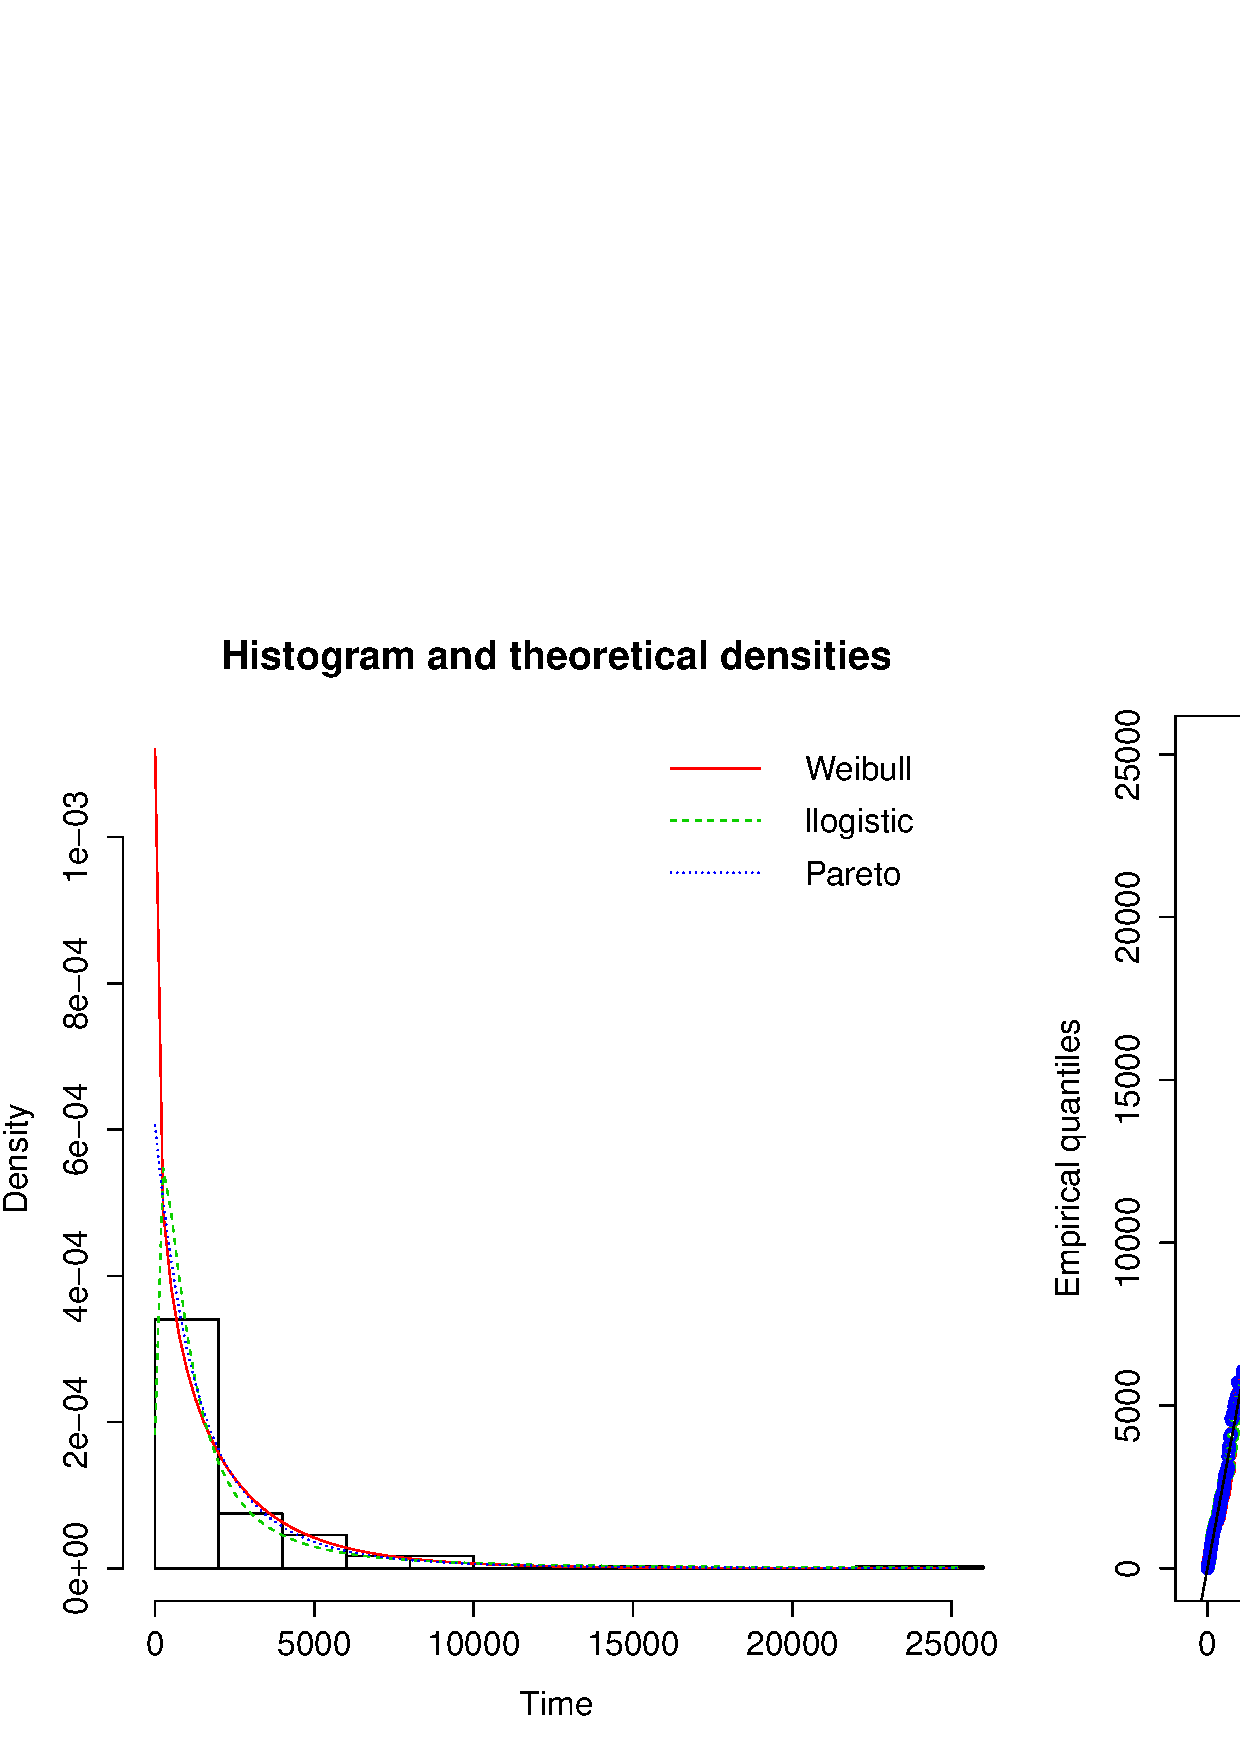
\includegraphics[height=5cm, width=14cm]{graphs/social_test/graph1.pdf} 
\caption{\% Field defects by severity}
\end{center}
\label{fig:socialtestdefectimpact}
\end{figure}

Fig. \ref{fig:socialtestdefectimpact} shows the percentage of the total defects broken down by severity. Minor defects are the most common with critical defects being the least common.



\begin {table}
%\caption {\% Field defects by impact} 
\caption {\% Field defects by impact}
\begin{center}
\begin{tabular}{l*{3}{c}r} Severity & Critical & Major & Minor \\ \hline \% of Total  & 2.9\% & 27.5\% & 69.5\% 
\end{tabular}
\end{center}
\label{tab:socialtestdefectimpact}
\end{table}


Field defects were classified by impact, which are shown graphically in Fig. \ref{fig:socialtestdefectimpact} and textually in Table \ref{fig:socialtestdefectimpact}.  These show the percentage of all defects of each severity type. The majority of defects found by the customer had a minor impact on their user experience (approximately 70\%), while approximately 28\% of users experienced a major severity defect and the remaining defects (just under 3\%) were of a critical severity.

\subsection{Results - defect component}

Fig. 2  shows the percentage of the total defects broken down by component and their severity. In each component minor defects are the most common with critical defects being the least common.

\begin{figure}
\begin{center}
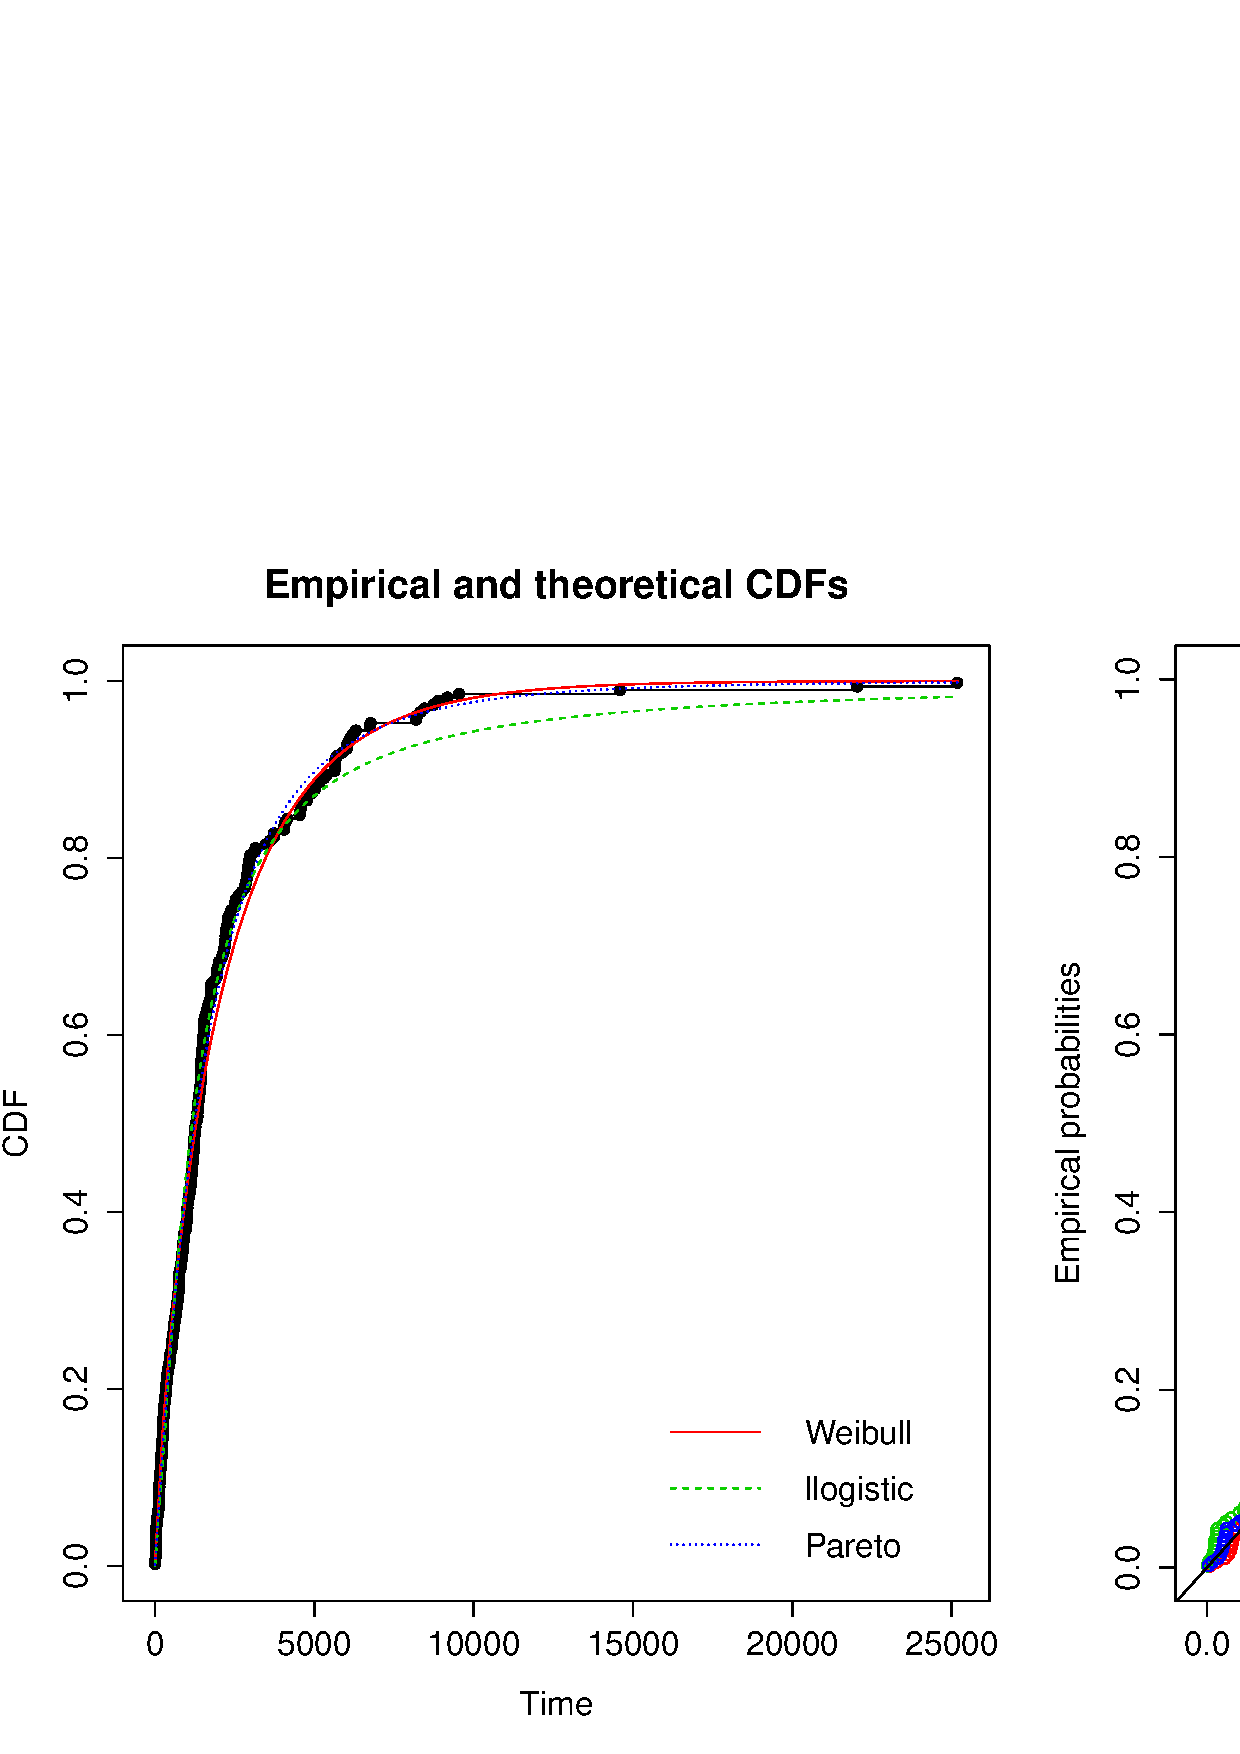
\includegraphics[height=5cm, width=14cm]{graphs/social_test/graph2.pdf} 
\caption{\% Field defects by component and severity}
\end{center}
\label{fig:defectcomp}
\end{figure}


\begin {table}[]
\caption {}
\caption {\% Field defects by component and severity} 
\begin{center}
\begin{tabular}{l*{5}{c}r} Severity & Critical & Major & Minor &  Total \\ \hline BSS & 0.5\%	& 5.7\% & 15.2\% & 21.4\% \\ Collaboration &	0.4\% & 3.5\% & 7.5\% & 11.4\% \\ Email	& 1.1\% & 5.2\% & 20.2\%	 & 26.5\%  \\  Social	& 1.0\% & 13.1\% & 26.5\% & 40.6\% \end{tabular}
\end{center}
\end{table}


TABLE II. Shows the percentage of all field defects broken down by component and severity. The Social application contained the most defects (41\%), Email (27\%) and BSS (21\%) had a broadly similar level of defects, and while the collaboration application had the least percentage number of defects found with 11\%.  The customer was most likely to find a minor severity defect irrespective of component used.

\subsection{Results - data centre location}

Fig. 3 shows the percentage of the total defects broken down by Data Centre and severity. In each data centre minor defects are the most common with critical defects being the least common. Previously it was noted that both centres A and C are high and medium usage, while data centre B is low usage. Given the level of field defects found in each data centre this supports the logical concept that higher usage leads to a greater number of defects.

\begin{figure}
\begin{center}
\includegraphics[height=5cm, width=14cm]{graphs/social_test/graph3.pdf} 
\caption{\% Field defects by data centre and severity}
\end{center}
\label{fig:defectdatacentre}
\end{figure}

\begin {table}
\caption {}
\caption {\% Field defects by data centre and severity} 
\begin{center}
\begin{tabular}{l*{5}{c}r} Data Centre & Critical & Major & Minor &  Total \\ \hline A & 1.6\%	 & 13.6\%	& 39.8\%	& 55.0\% \\ B & 0.7\% & 5.6\% & 7.3\% & 13.6\% \\ C & 0.6\% & 8.3\% & 22.4\%	 & 31.3\%   \end{tabular}
\end{center}
\end{table}


TABLE III. Breaks down the Field defects by data centre and by severity.  55\% of all field defects found were in data Centre A. data centre C recorded 31\% of defects, while data Centre B recorded only 14\% of defects. 

\subsection{Results - defect type}

Fig. 4 shows the percentage of the total defects broken down by testing type and severity. It was expected that minor severity would feature significantly, it's interesting to observe that the majority of functional defects are minor in nature. It was observed that for defects classified as System that the number of major and minor defects are practically the same. Finally it was noted that the customer did not find very many Performance defects. However of the defects that were found, slightly more were major than minor severity.

\begin{figure}
\begin{center}
\includegraphics[height=5cm, width=14cm]{graphs/social_test/graph4.pdf} 
\caption{\% Field defects by test type and severity}
\end{center}
\label{fig:defecttesttype}
\end{figure}

\begin {table}
\caption {}
\caption {\% Field defects by defect type and severity} 
\begin{center}
\begin{tabular}{l*{5}{c}r} Field Defect Type & Critical & Major & Minor &  Total \\ \hline Functional & 2.4\%	 & 21.8\%	& 64.3\%	& 88.5\% \\ Performance & 0.1\% & 0.7\% & 0.4\% & 1.2\% \\ System & 0.5\% & 5.0\% & 4.7\% & 10.3\%   \end{tabular}
\end{center}
\end{table}


TABLE IV shows the percentage of field defects found according to their type. 89\% of all customer issues reported were functional in nature, a further 10\% of customer defects were related to end to end system issues, while only 1\% of defects found were related to performance of either client interface or underlying server system. 


\subsection{Discussion - defect impact}

To answer the question how do field defects impact the customers overall user experience, Fig. 1 and TABLE I, clearly show that the customer finds more minor defects than any other type, almost 70\%. This means that the customer will come across some unexpected behaviour which does not result in data loss during their day to day product usage. Given that minor severity defects are found most often, the logical conclusion is that these types of defects are found by the customer exercising the most common component use cases. With the level of major defects found being 28\%, this also shows that these defects were found as part of a typical customers day to day usage, albeit to a lesser degree than minor defects. Clearly as part of the customers typical use case, they did encounter some form of data loss or non-trivial unexpected behaviour. With approximately 3\% of field defects being critical, this suggests that the likelihood of a customer experiencing a total component or some system wide failure is a rare event. That said customers, either by themselves or in conjunction with other users, were able to bring about behaviour, which impacted the wider system. \par

Given the nature of CD, it is important to point that new code and features are released frequently. Therefore by it's nature new field defects are raised on a continuous basis once new features are delivered. If a bug bounty program were introduced to incentivise field defect discovery, it would be interesting to determine the increase in the velocity of field defects from the introduction of such a scheme. Typically bug bounties have been the preserve of security defect discovery. By rolling out such a scheme for field defect discovery in general, it would be valuable to both the software developer: to focus on testing code paths which lead to higher severity issues, while incentivising the customer to uncover lower priority defects.

\subsection{Discussion - defect component}

Examining defect component, gives an indication of where customers are likely to find defects within each component. \par
Fig. 2 and TABLE II highlight that, at a component level approximately 41\% of the field defects found were in the social component. A further 27\% found in the email component, with 21\% in the BSS component with a final 11\% found in the collaboration component. While defect yields may not map directly to application usage (Unfortunately, no application usage metrics were available), conditional probabilities were calculated to determine like likelihood of certain combinations of defect attributes being found. With minor field defects being raised most often, conditional probabilities  for each component at minor impact level were calculated. It was noted that  P(minor\textbar email) had the highest probability with 0.762, P(minor\textbar BSS) with 0.709, P(minor\textbar collab) with 0.660 and P(minor\textbar social) with 0.654. This tells us that the customer is more likely to find a minor impact field defect in the email component. \par

This may seem counter intuitive given that 41\% of field defects were found in social. It is concluded that given the lower level of major impact defects found in email increases the likelihood of a minor impact defect being found.  The logical conclusion is that the more a component is used the more defects are likely to be found by end users. It is proposed that for popular components (in our study email \& social) that have continuous feature releases, by incentivising the discovery of lower impact defects by the customer, can help in-house testing refocus their efforts on the major severity testing across all test disciplines in their key feature/components areas. 

\subsection{Discussion - data centre location}
Fig. 3 and TABLE III give an insight into field defect breakdown by data centre. As mentioned in section III, it is known that the level of usage varies from data centre to data centre, interestingly the customers of data centre A (High Usage) reported the highest number of field defects with 55\% while data centre C (Medium Usage) and data centre B (Low Usage) had 31\% and 14\% defects raised respectively. Clearly there may be some form of correlation between concurrent user population and field defects raised. \par

Checking conditional probabilities for each data centre for both minor and major defects, as follows P(Minor\textbar DC-A) and P(Major\textbar DC-A) gives 0.724 and 0.248 respectively. These conditionals state that the customer is more likely to find a minor defect within data centre A. For data centre B  the following conditionals were calculated; P(Minor\textbar DC-B) and P(Major\textbar DC-B), which gives 0.537 and 0.411 respectively. These conditionals tell a similar story to that of data centre A, that the customer is more likely to find a minor defect than a major one. It is conjectured that the customer use case on data centre B is different to that of the other two data centres. Further analysis should be employed by the in-house test teams, to ensure their test scripts cover the main customer use case in data centre B which generates major impact field defects. Finally checking P(Minor\textbar DC-C), P(Major\textbar DC-C) gives 0.714 and 0.265 respectively. These conditional probabilities are very similar to those of data centre A. Customers are almost three times as likely to encounter a minor impact defect on data centre C than that of a major impact field defect. \par

Overall it was found that that for high and medium usage data centres the likelihood of finding minor field defects was almost three times that of finding a major impact defect. For the low usage data centre the probability of finding a major impact field defect was broadly similar to that of finding a minor impact field defect. Finally the customer was less effective at finding high severity defects irrespective of the data centre used. \par

In the context of CD, the same code is released to each data centre; clearly customers are more likely to be impacted differently depending on data centre. Knowing the underlying customer data centre use case is key.
With knowledge of both data centre usage and field defect data, incentivisation schemes can be tailor-made according to data centre. One suggestion would be a bounty to target minor field defects on high usage data centres, while refocusing in-house resources to find more major impact defects prior to release. 


\subsection{Discussion - defect type}
Finally in order to understand which type of field defect that the customer typically finds, defect type was examined. This metric may be one of the most important in terms of this study. It helps underscore which class of defect the customer is proficient at finding. \par

Fig 4 and TABLE IV clearly indicate that functional defects are the most commonly uncovered by the customer with 89\% of all defects found being functional. Also of significance is the severity of these defects with 64\% being minor severity. Clearly functional defects typically present themselves in the form of user experience behaviour errors where the end user attempted an operation and the behaviour encountered was unexpected. It is also important to note that 10\% of all issues were system errors, typically these manifest themselves as unexpected behaviour during active concurrent usage. One can infer that system errors are less common than functional ones. It may also be the case that system errors do not readily manifest themselves to the end user in the same way as functional defects. \par

Performance defects ranked the lowest in overall defects found with only 1\% of all problems being attributed to performance defects.  This data suggests that either the performance of each component was adequately tested prior to release or that performance defects may be harder for the end user to measure and quantify once in the field.  \par

Clearly from a customer's perspective they are more likely to find functional defects as these issues are found within the UI, however the customer finds a greater proportion of lower impact functional defects. Additionally the customer was less effective at finding high severity Performance and System field defects. From a CD/CI perspective, a balance needs to be struck in terms of the features being released and their likely defect type yield. For backend server features in-house test teams can focus almost exclusively on Systems and Performance testing. For features with rich functionality in-house test teams can focus on use cases, which are likely to yield critical and major defects with some additional minor impact areas. \par

In terms of bounties, for releases with high functional content software developers could award triple / double and single prizes for critical, major and minor impact field defects respectively with the knowledge that adequate testing was conducted in-house for critical and major use cases. Similarly for releases with high System and Performance and low functional features, proportional bounties may be awarded.


\subsection{Case study 1 - bibliography}
Social Testing citations (outside of Background research go here. \cite{ref1}.

\section{Case study 2 - Eat your own dogfood}

Field defect studies have been shown to provide a useful way to infer gaps within in-house testing \cite{sullivan1991software}\cite{boehm2005software}. Such studies, in conjunction with our framework, can be adopted by micro teams and SMEs to determine common failure types. \par 

The study presented in this paper examines approximately 2000 defects (both field and in-house) from a large cloud based real-time collaboration system. The data was collected over a 22-month period (Jan '15 -- Oct '16) and is comprised of three main components: Instant Messaging, Web Conferencing and an interactive audio and video component. \par

There are four in-house test teams whose functions are to find software defects; Function test, Performance test, Security and System test. Defects are also found by Development, DevOps, Support, Accessibility and well as other general users. Field detects are found by either the customer or any of the in-house teams just mentioned. Defects are typically of one of four types: Functional, Performance, Security and System. Defect severity is categorised as either: Critical, Major or Normal. The systems have been deployed within three data centres and are used by customers globally. The software is developed in Java and runs on Linux. Each release takes place on a Saturday.  \par 

Product development follows a continuous delivery (CD) model whereby small amounts of functionality are typically released to the public approximately every four to six weeks. For each defect we have access to the full report, but we particularly focus on the defect severity, defect type and found by whom. \par

This study aims to answer the following questions. First, what group is most likely to find either an in-house or field defect based on defect severity and test type? Second, what is the field defect discovery rate during the first fourteen days of a release? In order to answer these questions our study is divided into the following two subsections: defect discovery probability by team and field defect discovery rates. \par

\subsection{Defect discovery probability by team}

A question to software companies is, what types of defect are found both internally and externally. Similarly, what are the most common severity types found in-house and in the field? By analysing the types of defects found both internally and externally, a map can be built to determine which teams are most effective at finding a particular class of defect. Likewise for defects found in the field a similar map can be drawn to determine what types of defects a customer is good at finding. Given the limited resources of both micro teams and SMEs, an intersection of both maps could be used by internal test organisations to a) realign their test organisation to discover more defects and b) pivot internal test practices to more customer based usage patterns. \par

\subsection{14/28 days later -- defect discovery rates}

Studying when defects are found in the field gives us knowledge of how reliable software is. In the field of system
reliability, there is the idea that failures (defects) may follow a specific pattern which can be represented in the form of a `bathtub curve' \cite{klutke2003critical} \cite{wikipediabathtub}. The patterns can be summarised as follows: 1) Decreasing failure rate (early failures), 2) Constant failure rate (random failures) and 3) Increasing failure rate (wear-out failures). Of interest is to understand if field defects failures found within the first twenty eight days conform to
these characteristics. Of additional interest is to understand what types of defect (and their associated severity) occur
within the first two weeks of a release. \par

\subsection{Limitations of dataset}

The dataset has a number of practical limitations, which are now discussed. While the defect tracking system allows
for a granular categorisation system, whereby field defects can be mapped to a specific release. There were a number of field defects, which were mapped to an incorrect release. The authors used the defect creation date to determine which field defects belonged to which release. \par

The defect reports that form part of this study are from an enterprise Cloud system. As a result the analysis may not be relevant outside of these fields. \par

\subsection{Results - defect discovery probability by team}

Fig. 1 shows a bubble plot of in-house defect detection probability grouped by team type and defect severity. The size of the bubbles are scaled relative to the probability. The greater the probability the larger the bubble diameter. We also
show a probability by combined defect severity. The System test team have highest probability of finding a normal or major defect. System test are also most likely to find a defect of any severity. Function test are most likely to find critical defects.


\begin{figure}
\begin{center}
\includegraphics[height=5cm, width=14cm]{graphs/dogfood/Graph1.png} 
\caption{In-house defect severity detection probability (By Team)}
\end{center}
\label{fig:inhouselikesev}
\end{figure}

Fig. 2 shows a bubble plot of in-house defect detection probability grouped by team type and defect type. We also
show the probability of all defect types. The System test team have highest probability of finding a System, Functional and combined defect type. The Performance team are most likely to find a performance defect. Likewise the Security team are most adept at finding security defects. 

\begin{figure}
\begin{center}
\includegraphics[height=5cm, width=14cm]{graphs/dogfood/Graph2.png} 
\caption{In-house defect type detection probability (By Team)}
\end{center}
\label{fig:inhouseliketype}
\end{figure}


Fig. 3 shows a bubble plot of field defect detection probability grouped by team type and defect severity. We also show
a probability by combined defect severity. The customer is most likely to find a defect of any given severity in the field.

\begin{figure}
\begin{center}
\includegraphics[height=5cm, width=14cm]{graphs/dogfood/Graph3.png} 
\caption{Field defect type detection probability (By Team)}
\end{center}
\label{fig:fieldliketype}
\end{figure}


Fig. 4 shows a bubble plot of field defect detection probability grouped by team type and defect type. We also show a
probability of all defect types. The Customer is the most likely group to find any a defect of any given severity in the field.


\begin{figure}
\begin{center}
\includegraphics[height=5cm, width=14cm]{graphs/dogfood/Graph4.png} 
\caption{Field defect type detection probability (By Team)}
\end{center}
\label{fig:fieldliketype}
\end{figure}


\subsection{Results - 14/28 days later -- defect discovery rates}

Fig. 5 shows a line plot of percentage field defects raised during the first fourteen days of a release. The percentage values are an aggregate over the entire fifteen releases studied. Additionally the percentages are calculated as follows: an aggregate daily rate divided by the total number of field defects found. Days five and seven saw the highest aggregate percentage of field defects raised, while days eight and nine saw the lowest aggregate percentage
field defects detected.

\begin{figure*}
\begin{center}
\includegraphics[height=5cm, width=14cm]{graphs/dogfood/Graph5.png} 
\caption{\% aggregate field defect detection rate (First 14 days of a release)}
\end{center}
\label{fig:fieldliketype}
\end{figure*}


Fig. 6 shows a bar plot with fitted curve of percentage field defects raised during the first four weeks of a release. The percentage values are an aggregate over the entire fifteen releases studied divided by the total number of field defects found in the first twenty eight days of a release. Week one saw the highest number of field defects raised with just over 31\%, while weeks two and three had near identical rates with approximately 21\%, while week four had an increased rate (over weeks two and three) of almost 27\%.


\begin{figure}
\begin{center}
\includegraphics[height=5cm, width=12cm]{graphs/dogfood/Graph6.png} 
\caption{\% aggregate field defect detection rate (By week)}
\end{center}
\label{fig:fieldliketype}
\end{figure}

\subsection{Discussion - Defect discovery probability by team}

As mentioned in Section VI, we wanted to understand, for in-house defects, how defect detection was distributed across each internal test team by defect severity and type. Fig. 1 shows that the System test team was more likely to find both Normal (0.28) and Major (0.15) severity defects while the Function test team was slightly better at finding Critical defects (0.06). Overall the System test team were more likely to find a defect when we collapsed severity into a combined severity ranking (0.48). \par 

Interestingly, for defect type Fig. 2 illustrates that, the System test team were most likely to find System and 
Functional defects (both 0.23), while the Performance and Security teams found the most performance and security
related defects. Overall when all defects types are reduced to a single category the System test team are most likely to find a defect irrespective of type (0.48). \par

Fig. 3 shows that the customer is most likely to find a defect in the field, irrespective of severity (0.81). It's worth noting that for normal severity defects the customer has a probability of 0.58 while the next highest is the development team with a probability of 0.05.\par 

Fig. 4 highlights that the customer is highly skilled in detecting functional defects (0.77) and has a low probability
of finding other types of defects: Performance (0.01), Security (0) and System (0.03). For non functional defects, internal consumers (i.e. test teams) do find ``field defects'' as part of their daily usage of the software. Development (0.01 System defects) and DevOps (0.01 Performance and System defect types). \par 

A number of interesting points are raised by analysis of both sets of defect data. Firstly that the \emph{System test team have the highest probability of finding a defect in-house when severity or type are reduced to a single category}. What is surprising though is that while the \emph{Performance, Security and System teams are most adept at finding homogeneous defect types}, the \emph{Function test team is less likely to find a Functional defect (0.19) compared to System Test}. It is worth noting that the Development team are also quite skilled at flushing out functional defects too (0.13). Second that the Customer is more likely to find a field defect than internal users ``Dogfooding'' their own software. That said, the customer appears to find a very specific type of defect, a normal severity functional defect.  \par 

Given the overlap in terms of detection of Functional defects there is an argument to merge both Function and System test teams into a single group. Based on the dataset we know that the System test team are skilled at finding functional defects, by merging teams there would be the added benefit of upskilling the functional team members to test and detect System defects. Furthermore, it makes sense to have a separate team to test both the Performance and Security areas of the product because this testing requires specialist knowledge which enables these test teams to focus on their core areas of expertise. \par

With the customer being so adept at flushing out normal severity functional defects, focus instead should be placed on determining what test paths should be included in future test cases to capture these classes of functional defects as part of an internal testing. However the customer should be incentivised in some manner for the number of lower severity defects they find. We discuss this subject matter in more detail in prior work \cite{7331827}.

Finally, irrespective of the dataset and the results tied directly to it, we suggest the following outcomes for our framework: a) test teams should be aligned based on the types of defects they find, b) in-house testing should prioritise test paths to areas of the product, which are both critical path and where the customer is least likely to find a defect and c) schemes to incentivise the customer to find low severity defects could be introduced. \par

\subsection{Discussion - 14/28 days later -- defect discovery rates}

Examining the field defect discovery rate during the first twenty eight days of release helps us to understand what types of defects a customer is likely to find. \par 

Fig 5. shows the percentage of defects found the first fourteen days of a release. Looking at the
`All Defects' line initially we can clearly see that field defect detection peaks at day five. Approximately 6\% of all field
defects (raised in the first twenty eight days of a release) were found on the fifth day of a release. The second highest
daily rate appears on day seven with 4\%. Also of note is that, on days eight and nine, we observed the least number
of field defects raised (0.13\% \& 0.27\% respectively). This may be attributed to both of these days falling on a weekend. That said the first two days of a release also fall on weekend and see a higher rate of field defects raised (Approximately 2\% on both days). Finally as part of the second working week of a release the rate rises to approximately 3\% and remains steady at this rate for the remainder of the second week. \par 

Another point of interest is evident in Fig. 5. If we consider Normal \& Major severity, Functional type and Customer
found field defects we can see how close these lines mirror the overall rate line. This confirms our intuition that these
categories of field defect are highly correlated as part of the overall data set. Our reason for this belief is that, these four categories of defect contribute a significant proportion to the overall dataset. No formal regression analysis has been conducted to confirm our intuition. \par 

Fig 6. Presents a bar plot with fitted spline curve. This plot illustrates the percentage of field defects raised weekly during the first twenty eight days of a release. Clearly we can see that the highest percentage of field defects detected within the first month of a release are found in the first week of a release. 31\% of all field defects found in the first month of a release are found during the first seven days. Also of note is the rate drop during weeks two and three of release, approximately 21\% for both weeks. Finally it is worth noting that the rate increases to approximately 27\% during week four. \par 

Looking through the lens of analysis from both a fortnightly and monthly perspective, we can clearly see that highest
percentage of field defects are found within the first seven days of a release (specifically day five). There may be a host of reasons why the customer finds so many defects in such early stage of a release: Poor customer usecase profiling, lack of test automation, lack of test resources. Irrespective of the root causes it is worth noting that the majority of field defects the customer uncovers are low severity and functional. Therefore a targeted set of crowdsourced tests would be useful in flushing our additional defects prior to public release. \par 

In Section III we mentioned the idea of software reliability and how the `bathub curve' is used (at a high level) to illustrate the three stages of system reliability. We observed in Fig 6. the weekly percentage rate of field defect discovery. We noted the high initial rate in week one, the drop in weeks two and three and finally the increased rate in week four. This behaviour can be mapped directly to the early, random and wear-out (i.e. failure that occur due to sustained usage) failures, which characterise reliability. Targeted survival analysis of field defects found in the first month of a release is required to determine whether field defect do indeed contain early, random and wear-out attributes. We temper this finding with the observation that there is an baseline of at least 20\% failure rate on any given week.\par 

In future SMEs and micro teams can adopt a two week crowdsourced--dogfood test program prior to release to the
general public. By leveraging the power of both the internal work force and a crowdsourced test cohort for a fixed duration, companies can uncover many `field' defects prior to general release. Certainly this crowdsourced--dogfood program will uncover many defects with early and random characteristics. Based on the analysis of in-house test data, these types of defect are difficult to uncover as part of internal testing. For defects with wear-out attributes by adopting a framework of survival analysis, teams can determine if there are specific component which wear out more quickly than others. With this knowledge development teams can adopt remediation plans to ensure their components are more robust to wear-our failures. \par

Putting the findings drawn directly from our dataset to one side, we can add the following proposals to our framework: a) a period of crowdsourced-dogfood testing should be conducted for a two week period prior to release, b) the crowdsourced team should contain individuals from a variety of backgrounds.

\subsection{Case study 2 - bibliography}
Dogfood citations (outside of Background research) go here. \cite{ref1}.


% % % % % % % % % % % % % % % % % % % % % % % % % % % % % % % % % % % % % % % % % % % % % % % % % % % % % %
%------------------------------------------- CONCLUSIONS --------------------------------------------------
% % % % % % % % % % % % % % % % % % % % % % % % % % % % % % % % % % % % % % % % % % % % % % % % % % % % % %

\section{Conclusion}

** Social Testing ** \par 

Previous studies have shown that analysis of field defects is a valuable exercise. Additionally that bug bounty rewards provide an incentive to end users to improve software quality once in the field. The purpose of this study was to examine the role of the customer in the generation of field defects. It was found that the customer was quite adept at finding minor severity functional defects.  The findings of this study support previous work particularly in the gaps between in-house software testing and general customer usage. \par

This work provides a more detailed study in relation to software developed using a CD model. Adoption of CD means continuous feature releases and continuous defects, however feature releases can be delivered in such a away to ensure that there is not a significant burden on in-house test teams.  \par

 In future SME's can assess their field defect data to understand the core gap areas in relation to defect impact, component, data centre and type. A specific test framework can then be built to allow SME's to focus on test areas, which are likely to yield high impact defects, and which may be difficult for an end user to discover. 
Furthermore by providing the customer with an incentivised scheme, in the form of bug bounties to find specific defects types will improve overall software quality through the iterative development and release process that is CD. 

** Social Dogfood ** \par

The purpose of this study was to examine in-house and field defects for a Cloud based collaboration application. We
found that Performance and Security defects are specialist focus areas which are best handled by specific teams. We also found a significant overlap in the area of Functional defects found by the System test team. Additionally the customer is skilled at finding specific defects types (Normal Functional) in our data set. \par

Furthermore we found that field defect detection occurs most often in the first seven days of a release and that over a
monthly period field defect detection rates mirror those seen in other fields of reliability engineering. \par

In future SMEs can align in-house test teams to overlapping test areas to help focus test effort. Additionally for field defects of high severity re-focusing of test plans to high impact areas can mitigate their detection in the field. A reward/gamification framework can be introduced to customers who find low severity defects in the field. Likewise a co-ordinated system of crowdsourced dogfood testing can be implemented prior to release, to reduce the number of defects found in the first two weeks of release.\par





% ---------------------------------------------------------------------------
% ----------------------- end of thesis sub-document ------------------------
% ---------------------------------------------------------------------------
